\chapter{Noise detection and reduction}

One common approach is to compare the current frame with the previous. This is useful in video compression, when it is necessary to evaluate the changes and write only changes rather than the entire frame. But this is not the best way to detect movement. At this stage, we obtain the image with the white pixels in the place where the current frame It differs from the previous frame to said threshold value. It can already be considered pixels, and if the amount is greater than a predetermined alarm level we can signal motion events.

\section{Human body detection}


At this stage, we obtain the image with the white pixels in the place where the current frame It differs from the previous frame to said threshold value. It can already be considered pixels, and if the amount is greater than a predetermined alarm level we can signal motion events.

But most cameras do noisy images, so that we get movement in places where there is no movement at all. On this issue I wrote above.

There is another approach. It is possible to compare the current frame with no previous, but with the first frame of a video sequence. Thus, if not were objects in the initial frame, the comparison of the current frame from the first one will give us a moving object, regardless of its speed. But this approach has a big drawback - what will happen if there is, for example, the car for the first frame, and then he was gone? Yes, we will always have a motion detected in the place where car was. Of course, we can extend the initial frame sometimes, but it will not give good results in those cases where we cannot guarantee that the first frame contains only the static background. But perhaps the opposite situation. If I I put a picture on the wall in the room? I get motion detect only the initial the frame will be resumed.

Most efficient algorithms based on the creation of the so-called background and comparing each scene of the current frame with the background.

Upon completion of the process of filling the frame with black and white dots begins the process of selecting objects. Bunches of white pixels algorithm incorporates one the object and makes it stand out on the screen rectangle. 

There exists another solution like HOG (Histogram of Oriented Gradients) - descriptors singular points, which are used in computer vision and image processing for the purpose of object recognition. This technique is based on counting the number of lines of gradient in the local areas of the image. This method is similar to the edge direction histogram, SIFT descriptors and contexts shape, but is characterized in that calculated on a dense grid of uniformly distributed cells, and uses local contrast normalization overlapped to increase accuracy.

The basic idea of the algorithm is the assumption that the appearance and shape of the object on the image area can be described by the distribution of intensity gradients or edge directions. The implementation of these descriptors can be made by dividing the image into small connected regions, called cells, and the calculation for each cell of the histogram or gradient direction towards the edges of the pixels inside the cell. The combination of these histograms and a handle. To increase the accuracy of the local histogram undergo normalization in contrast. To this end, the measure of the intensity calculated for the large fragment of the image, which is called a block and the value obtained is used for normalizing. Normalized descriptors have better invariance with respect to the coverage.

HOG descriptor has several advantages over other descriptors. Since HOG working locally method supports the invariance of geometric and photometric changes, except for the orientation of the object. These changes will only appear in their increased image fragments. Moreover, as found Dalal and Triggs, rough partition of the space, the exact calculation of areas and strong local photometric normalization allow ignore pedestrians, if they support the vertical position of the body. Descriptor HOG, therefore, is a good way of finding people in the images.

The first step in many computing detectors singular points is the normalization of the colors and gamma correction. Dalal and Triggs found that HOG descriptor for this step can be omitted, as the subsequent normalization will give the same result. Therefore, the first step is calculated gradients. The most common method is to use a one-dimensional differentiating mask in the horizontal and / or vertical direction. This method requires a filter or a color luminance component by using the following filter kernels:

Dalal and Triggs use more complex masks such as Sobel 3x3 (Sobel operator) or diagonal masks, but the masks have shown lower performance for the task. They also experimented with a Gaussian blur to the application of differentiating mask, but also found that skipping this step increases the speed without noticeable loss of quality.

Grouping directions. In the next step the cells histograms are computed. Each pixel in a cell involved in the weighted voting for the channel histogram of directions based on the value of the gradient. The cells may be rectangular or circular shape, the channels are uniformly distributed histogram from 0 to 180 or 0 to 360 degrees, depending on the calculated "sign" or "unsigned gradient". Dalal and Triggs found that unsigned gradient together with nine channels of the histogram gives the best results in the recognition of people. The allocation of voting weights in the weight of the pixel can be specified either absolute value of gradient, or some function of him; in real tests the absolute value of the gradient gives the best results. Other possible embodiments may be the square root, square or trim the absolute value of the gradient. \cite{Dalal}

Ji Xiaofei, Liu Honghai \cite{Yu} provides a complete survey of the human motion detection with changes in appearance-invariant expression, and identifying specific facial expressions and legal proceedings. The to help readers understand the combined development Visual analysis of human motion detection, paper gifts the recent rise in the detection of human vision, posture-invariant demonstration and evaluation, and human performance understanding. Public available standard sets of data recommended. Last replace evaluates the development so far, and outlines some of the observed problems and future guidelines, and Deciding what you need to get the objectives of the common man Expertise movement.

\section{Motion detection}

Motion detection plays a fundamental role in any monitoring object or video Algorithm observation to such an extent that almost all such algorithms begin with the movement Detection. In fact, the reliability with which potential foreground objects in motion may be identified directly affects the efficiency and performance achievable subsequent processing steps of tracking and / or detection of objects. Nevertheless, the detection of changes in regions of images of the same scene and not just The problem, as it not only depends on the characteristics of the foreground, but also on the characteristics of the background, such as, for example, the presence of oscillating elements. So, in this chapter, we have focused on the problem of motion detection in the basic case, ie when all the elements of the background still. The goal is to address various issues related to the use of different image sensors, adapting to different environments, with different speed, changes shape purpose, or some uncontrolled dynamic factors, such as, for example, incremental / sudden changes in lighting. Thus, firstly, a brief review of previous related approaches an analysis of the factors that can make the system fail. Then we propose segmentation algorithm of movement, which has successfully engaged all having problems. \cite{Dzung}

Motion detection is fundamental to any object tracking or surveillance algorithm, to such an extent that almost all such algorithms begin with the detection of motion. In fact, the reliability with which the potential foreground objects in motion can be identified directly affect the efficiency and performance level achievable for subsequent processing steps of tracking and / or recognition. Nevertheless, the detection of Regions of the changes in the images of the same scene is not an easy task, as it depends not only on the characteristics of the priority elements, but also on background characteristics, such as, for example, the presence of oscillating elements.\cite{Chen} In this chapter we will study the motion detection in the static scenes, that is, only the elements of motion is goals. Thus, it is possible to analyze and solve issues regarding the use of different image sensors, adaptation different environments, and in certain dynamic, uncontrolled factors such as (Gradual or global) changes in lighting. From this starting point, any detected change pixel will be considered as part of the foreground object. For this reason, methods based on the time information using frame difference threshold can be set. By depending on the time it means a ratio between frames, in contrast, two different approaches it is defined. On the one hand, the pattern (-frames) Subtraction uses the reference frame represent the background scene. This frame is usually mounted on the first captured Image. Thus, the pixel is classified as foreground if the current value is significantly different from its value in the frame. While this may seem like an ideal the solution should be noted that two distinct situations may occur in real conditions 

\begin{enumerate}
    \item Ideal situation. Therefore in the frame. In that Case, the resulting image will be the same as a desired segmentation result
    \item The overall situation. Priority objects can appear in the frame. Their making the presence of background subtraction fail by giving false positives due their position in the frame. \cite{Cheung}
\end{enumerate}


To solve the problem of localization, identification and further analysis of the dynamic movement of objects in the images it has been proposed and implemented two approaches. The first approach is based on the segmentation of motion, and can be arbitrarily assigned to the algorithms of the primary level, does not use the context and models. The second approach requires a model of possible objects in the scene and its immutable background. It uses the statistical parameters of the background obtained in the primary level image analysis.
The simplest segmentation algorithms applied pointwise threshold qualifier: background, if the change in the brightness of the image at a given point in time is less than a certain value, and the object - otherwise.
In a number of these cases, these algorithms do not work: 
\begin{itemize}
    \item background includes segments with oscillating brightness (for example, trees in windy conditions);
    \item global change of scene illumination (cloudiness);
    \item local change in light background (shadow);
    \item moving object is a uniform color.
\end{itemize}

To overcome such difficulties in motion segmentation algorithm was proposed to use the simplified optical flow function g (x, y, t), instead of a simple function of the time derivative of the brightness point.

For a more effective analysis (for example, to eliminate artifact segments oscillating brightness) proposed to use as a medium-term and long-term function of the history of changes. Both as a medium-term and long-term function of two-component. The first component is an averaging function g (x, y, t) for the selected time interval and a second average deviation. Thus, the discriminant function "object - background" is expressed as a logical (non-linear) superposition of previously obtained feature stories pointwise change the image.
Thresholds discriminant function set on the basis of the training program with the assistance of the test of dynamic images. For example, consider the oscillating changes in brightness point related to the periodic motion of the background. The correct choice of the averaging period oscillation damping effect. In this, as in so many problems tracking necessary initialization scene model (i.e. a period of time during which the program "learns" by choosing the desired settings).

Point-wise segmentation using the proposed discriminant function inevitably leads to occasional mistakes (analogue impulse noise in the image). To correct these errors is necessary to use detector "emissions". The paper proposed to use the detector on the basis of a gradient of connectedness.

In some situations it is not enough only time analysis of dynamic images. Global changes in scene illumination, plus local change light (ie not provided investigated the dynamic model of the scene, and, accordingly, the absence of such artifacts to test dynamic image), often leads to failure of the algorithm as a whole.

It is known that in such computer vision tasks, you can use the stereo image. Indeed, the situation with the classification of the background can be significantly simplified if possible to obtain three-dimensional information analyzed dynamic scene. In fact, the depth map of the scene does not depend on the time change in the illumination of the analyzed scene, and the change in the depth map of the scene is a great feature for traffic segmentation.
The problem is that the algorithms that compute depth map of good quality require considerable computational effort, which does not allow the use of such methods in applications that require tracking in real-time pace. To overcome such contradiction in the proposed use of the new stereo matching technique, which is described in detail in the publications. The proposed method is an analog stereo matching based on dynamic programming and, therefore, can be performed at a speed close to real time, while the proposed algorithm allows to calculate the depth map is much more accurate than improvable prototype.

The possibility of using the hybrid functions point-wise history changes as images and depth maps. That is, in the case where the classification using the discriminant function based on the point-wise brightness changes to errors, a classifier based on a function of the depth map change was correct. Computer experiments on the model of the complex automated tracking confirmed that in this case the motion segmentation algorithm is more efficient.
Most of the tasks of tracking, anyway, due to the segmentation and recognition of strictly defined moving objects, such as cars on the roads. Among these tasks special place occupied by the problem of tracking and identification of the nature of human movement. The object is achieved in several stages: first part of the image is classified as the object, then the object is classified as a human silhouette, finally, each time a specific position is recognized by human.

The problem is greatly simplified if the object of interest only to people. All other moving objects are classified as background. The presence of human movement model simplifies the task of classification of "object - background ', but in parallel there is a whole host of other problems. One of them - the verification of the model. It is assumed that an "agent" or tracking object can perform a limited number of simple actions, such as walking, running, jumping, etc. N. The sequence of postures that constitute a recognizable action verified silhouette motion segment. This problem is not unique in itself and can be solved with the involvement of the theory of probability and methods based on the use of Kalman filters. Each posture is characterized by a multidimensional vector uniquely characterizes the three-dimensional model of human skeleton. Removing the test statistics using dynamic images, greatly complicated by the fact that even one and the same person performs a specific action at different speeds. Therefore, the synchronization of various motion vectors required.
Previously, such a synchronizing manually. There is also an automatic synchronization technique key-frame, which does not work very reliably and often requires manual adjustment. In these studies, it was proposed and implemented a method of automatic synchronization dense. The main idea of the method is similar to that used with the concurrence of lines in the stereo. The proposed algorithm has been implemented in software and using showed high synchronization accuracy.

As a result of the research, a new approach to the analysis of dynamic images of static cameras, based on the history of point-wise function changes the picture. On the basis of the proposed approach has been implemented method of localization and extraction of "useful" information from the processed moving image. In the development of the synthesis method used statistical methods of classification of objects, as well as traditional methods of motion estimation of dynamic images. On the basis of the proposed method was created programming model of automated tracking systems, computer testing of the model showed a high efficiency of the proposed approach.


\section{Segmentation of moving objects in the video stream}

Finding and tracking moving objects in the video stream is an important task for applications such as security systems, the analysis of the traffic on the motorway, smart room, etc. Often the first step to solving these problems is to distinguish the foreground. This article will consider several methods to subtract the background (background subtraction), used to solve this problem. Methods background subtraction - are methods that build the background model at each stage and generate per-pixel block compares the current value in each pixel with the model in accordance with the comparison results deciding, the pixel belongs to the background or to the front. The article will describe the main challenges faced by these methods, and solutions will be discussed some of them.

Consider the simplest algorithm of subtracting background and his example look at the main problems faced by this kind of algorithms. We assume that the camera comes with a halftone image (if coming from the camera color images they obviously can lead to a semitone, such as using a formula). The algorithm preserves the first frame of the video sequence, and then for each of the next frame to the module uses the threshold current and the difference between the saved image for each pixel. So:

\begin{enumerate}
    
    \item Save the first image of the video sequence
    \item For each of the next frame when, where w and h are the width and height of a picture, respectively, then the pixel[i][j] considered the front-stage or it is considered background.
    \item In order to eliminate noise to the resulting binary image you can apply a median filter or the operation mat. morphology. \cite{Neri}
    
\end{enumerate}

Two kinds of errors such algorithm: front-stage pixel was classified as background (eg as a consequence of noise or due to the fact that the front-stage object color matches the color of the background) and background pixel was classified as a front-stage (eg because of the noise). By varying the parameter (threshold) and subsequent filtering parameters can adjust the sensitivity of the algorithm that is Levels of these errors. The apparent advantage of this algorithm is the exceptional ease of implementation and high performance. Despite these advantages there are several problems that make the algorithm practically inapplicable in practice.

Camera noise. Different camera noise in different ways and it can also be a problem for this algorithm background subtraction. Non-adaptive threshold has to be manually configured for different cameras and different camera settings in different ways, which of course is not desirable for the automatic systems.

\section{Shadow Detection}

Accurate detection and suppression of moving shadows is one of the main problems as background subtraction algorithms each moving object casts a shadow. This can lead to serious distortions in the shape of objects, and can also lead to the fact that different objects are merged into one, which can greatly complicate subsequent analysis and processing. The reader is invited shadow decreasing algorithm, using local (per-pixel) properties of the shadow.

Consider a point of the scene and let it has color, then after the fall of this shadow point it will have a color, where the coefficient determines how fallen illumination point. It turns out that this fact is enough to build a good system of suppression of shadows. shadow decreasing algorithm will be explained for RGB algorithm implementation with a single normal distribution, but the system similarly shadow decreasing can be integrated into an algorithm with a threshold and an algorithm with a mixture of normal distributions. Let - the background color in a pixel (ie, the estimate mat. Standby 3 dimensional random variable modeling the background in a given pixel) and - the current value of the pixel. First, go into the YUV color space that is . The YUV component Y determines the intensity and the components U, V determine the color. Thus a fall in the shadow of the object Y value should seriously reduced and the values of U, V virtually not change. Thus streamed value in the pixel is classified as a shadow when, where - the thresholds defining the sensitivity of the system shadow decreasing. Fig. 4 shows an example of the system for detecting shadows RGB algorithm implementation with a mixture of normal distributions. It is worth noting that this is not the only way to suppress the shadows using their local properties. In \cite{Cucchiara} we can read about a similar system that uses HSV instead YUV.


\section{Filtering}

In this group there was put methods that highlight areas of interest in the images without their analysis. Most of these methods are applied for a single transformation to all points of the image. At the level of filtering the image analysis is not performed, but the points that pass filter can be regarded as regions with special characteristics. The images generated by various opto-electronic systems and recorded with a variety of receivers are distorted by the influence of interference of various kinds.\cite{Gonzalez} Artefacts made all the components depicting device, starting with the lighting system (for example, non-uniformity of illumination of the subject). Distortion, which makes the optical system, known at the stage of its design and are called aberrations. Distortion, which make electronic receivers of radiation, such as CCD, called electronic noise. Interference difficult visual analysis of the image and its automatic processing.

The weakening of the action of interference is achieved by filtration. When filtering the brightness (tone) of each point of the original image, distorted hindrance, is replaced by some other luminance value, which recognized the least distorted noise. To perform the filtering is necessary to develop the principles of these transformations, which are based on the fact that the intensity of the image varies according to the spatial coordinates slower than the function of interference. In other cases, on the contrary, a sign of the useful signal are sudden changes in brightness.

The filtering methods in the evaluation of the real signal at some point in the frame to take into account a set (neighborhood) of adjacent points, taking advantage of a certain similarity of the signal at these points. The concept of neighborhood is quite conventional. The neighborhood can be formed only on frame closest neighbors, but may be a neighborhood containing enough and strong enough distant points of the frame. In this case, the degree of influence (weight) of the near and far points of the decisions made by the filter at a given point of the frame, will be completely different. Thus, based on the ideology of filtering data as a rational use of the operating point, and of its vicinity.

When the solution of filtration using probabilistic models and image noise and apply the statistical criteria of optimality. This is due to the random nature of the interference and the desire to obtain the minimum average difference between the processing result from the ideal signal. The variety of methods and algorithms of filtering associated with a wide variety of mathematical models of signals and noise, as well as the various criteria of optimality.

The simplest transformation - a threshold binarization image. For the RGB image and grayscale images is the threshold value of the color. There are common problems in which this conversion is enough. Suppose you want to automatically identify objects on a white sheet of paper. The example is described in Figures below. In Figure \ref{fig:original_for_threshold} is shown the original image. In Figure \ref{fig:image_after_threshold} is shown the result of binarization image.

\begin{figure}[h]
    \centering
    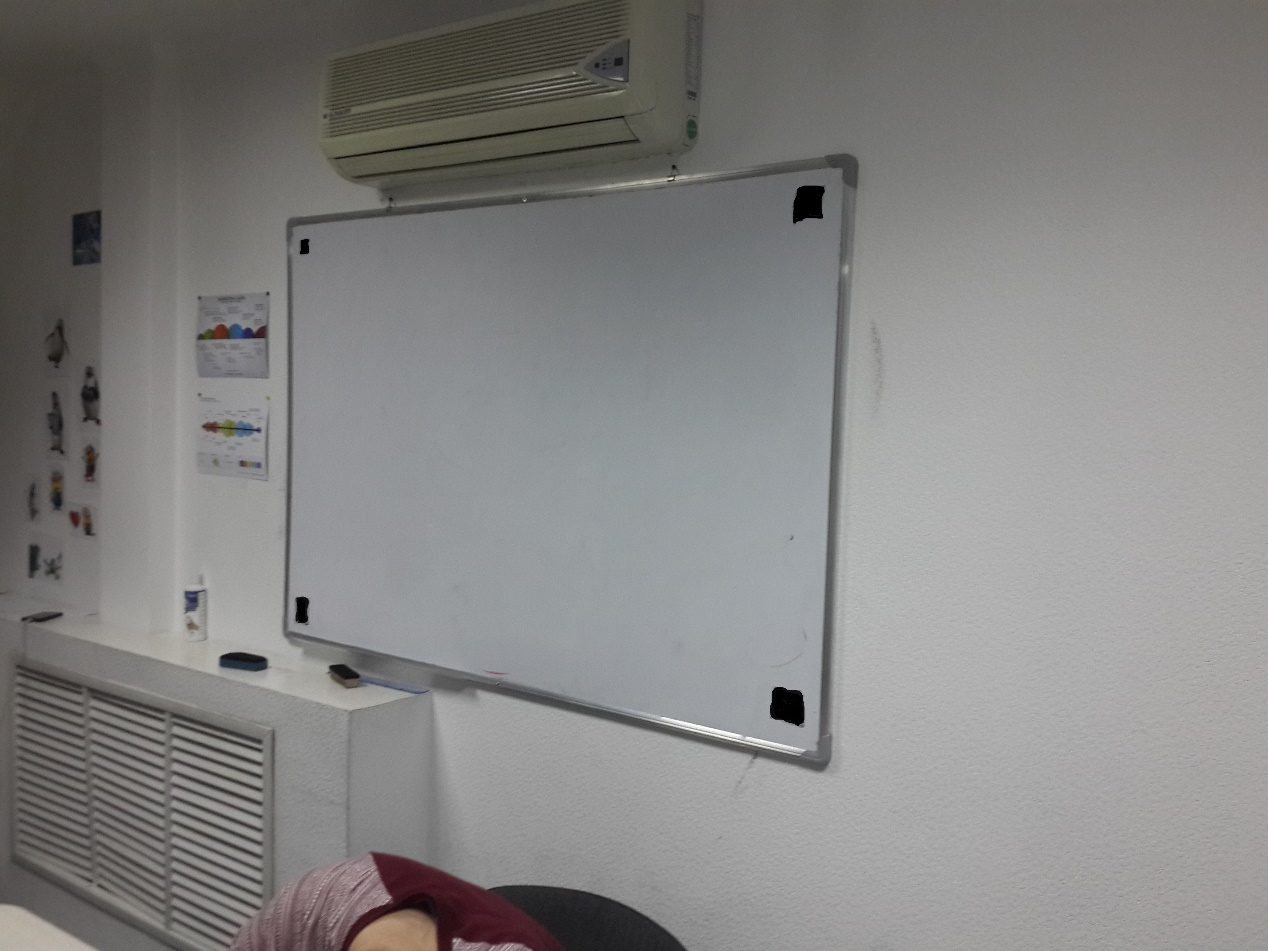
\includegraphics[width=0.7\textwidth]{Figures/original_for_threshold}
    \caption{Original image before binarization}
    \label{fig:original_for_threshold}
\end{figure}

\begin{figure}[h]
    \centering
    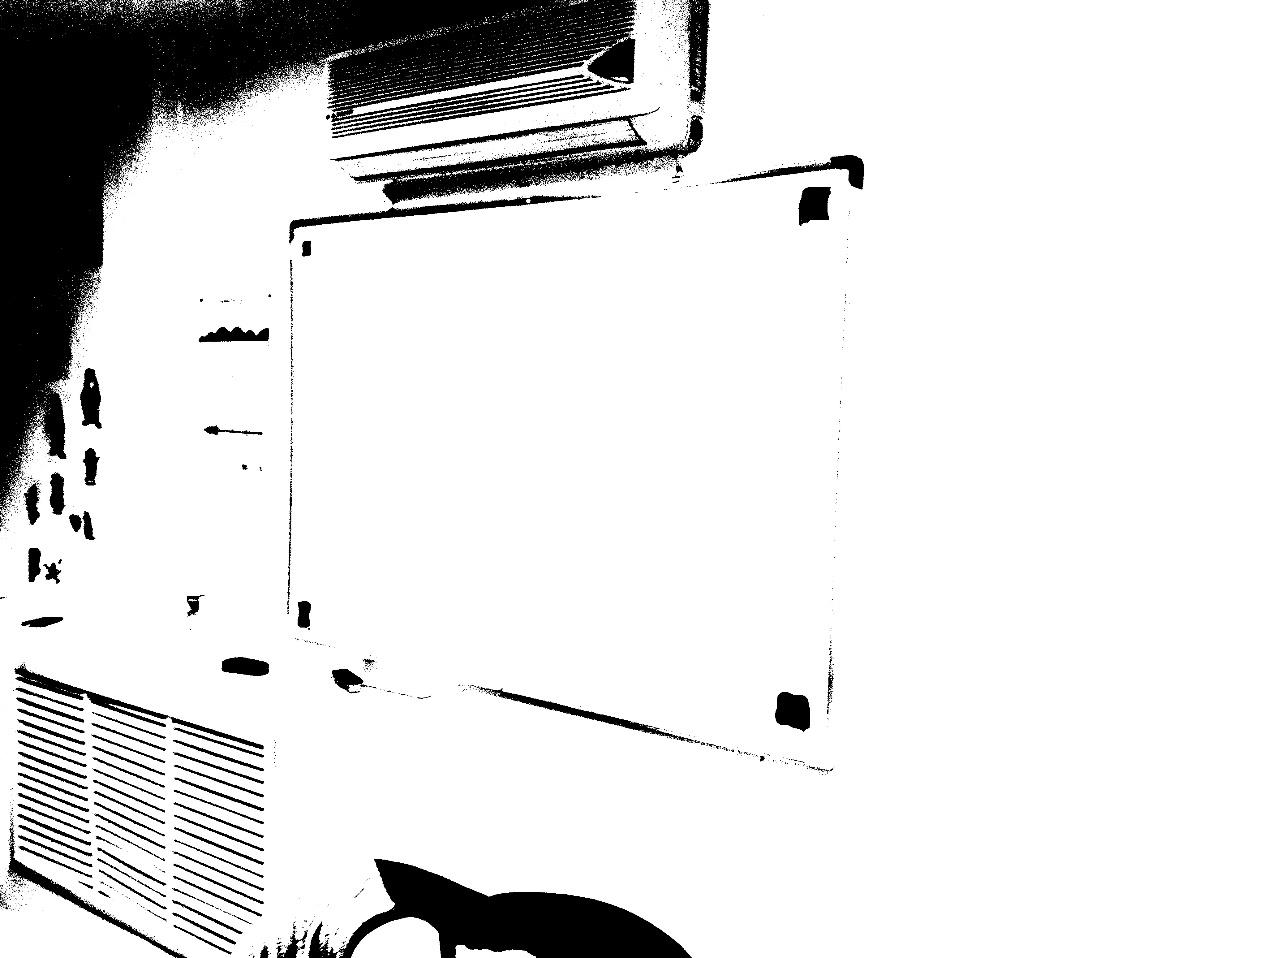
\includegraphics[width=0.7\textwidth]{Figures/image_after_threshold}
    \caption{Image after binarization with specified threshold}
    \label{fig:image_after_threshold}
\end{figure}

Selection of the threshold on which there is binarization, largely determines the process of the binarization. In this case, the image has been binarized by the average color. Usually, binarization is carried out using an algorithm which adaptively selects a threshold. So the algorithm can be a choice math expectancy or fashion. And you can select the highest peak of the histogram. The graphic is shown in Fig \ref{fig:histogram}

\begin{figure}[h]
    \centering
    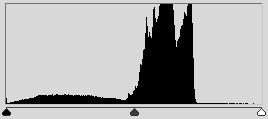
\includegraphics[width=0.7\textwidth]{Figures/histogram}
    \caption{Histogram}
    \label{fig:histogram}
\end{figure}


Binarization may yield very interesting results with histograms, including situations when we consider the image is not RGB, and HSV. For example, a segment of interest color. This principle can be constructed as a detector and the detector mark human skin

It is possible to make binarization to any image. But it would take more time to complete the binarization process because of the RGB image. In RGB there are three channels to work with. To make it more easier to binarization it would be good to make grayscale on image. Grayscale image turns image into one channeled image.

Grayscale - a reference image of a number of uniform optical density of the neutral-gray fields produced on the basis of transparent or opaque and designed to assess and measure the quality of Tone in the photographic recording, scanning, copying and printing processes. Gray scale brightness values often expressed as a percentage, with 0\% is white (no black pigment on a white background) 100\% - black (die deep pure black pigment)

In the computer representation of the gray scale is widely common uses for each pixel of the image is one byte (8 bits) of information. Such a scale transmits 256 colors (gradations) of gray color or brightness (value of 0 represents black, and 255 - white).

The gray scale intensity of reflected light at each pixel of the visible portion of the electromagnetic spectrum (see. Visible light).
The gray scale is used when converting grayscale images in color model. Since the gray scale is located on a diagonal in the color cube model RGB, then each component receives the same values equal to the values of shades of gray. In Figure \ref{fig:grayscale} you can see an example image result after grayscaling process.

\begin{figure}[h]
    \centering
    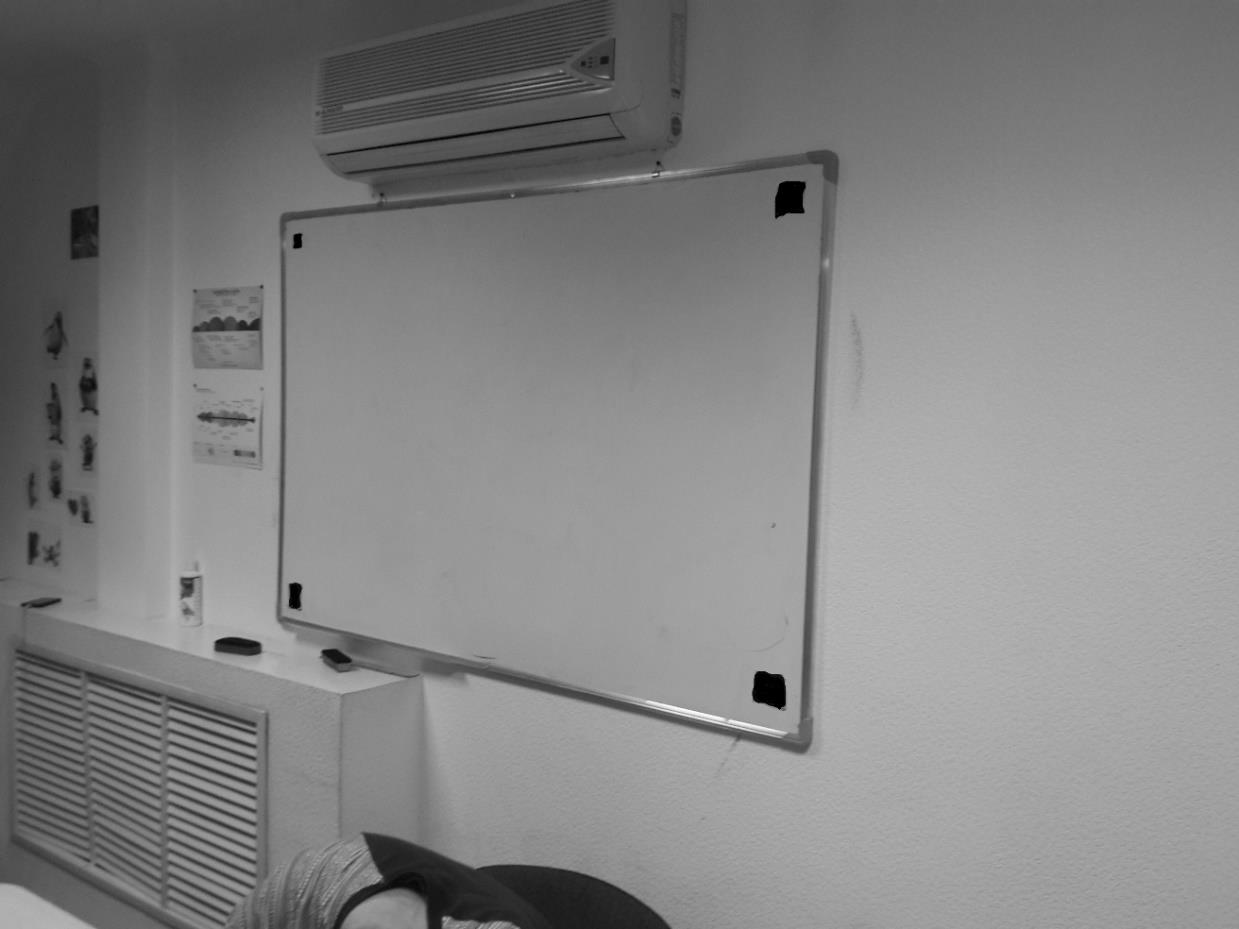
\includegraphics[width=0.7\textwidth]{Figures/grayscale}
    \caption{Grayscale}
    \label{fig:grayscale}
\end{figure}


Blur image plays an important role in modern computer graphics. Motion blur often directed to simulate nearsightedness (in cases where the myopia becomes desirable, or even necessary). So, blur parts of the image is often used for reasons of censorship. In some cases, the blur is an integral part of the various techniques of image correction aimed at addressing specific defects (excessive detail, scanning defects, scratches, dust). We know that the Model and photographers use special procedures blur photographic images to achieve the effect of "eliminating wrinkles." Blurred images are also more amenable to compression (for example, when you save a JPEG image file is smaller in size and less severe compression artifacts). Different techniques of image blur are available in all of modern graphics editors (such as Adobe Photoshop, The GIMP). One of the most important algorithms for image blur is t. N. Gaussian Blur.

Gaussian Blur - a characteristic blur filter, which uses the normal distribution (also called the Gaussian distribution, hence the name) to calculate the transformation applied to each pixel of the image. In two dimensions, this formula defines the surface having the form of concentric circles with a Gaussian distribution from the central point. Pixels where the distribution is different from zero are used to construct convolution matrix that is applied to the original image. The value of each pixel becomes a weighted average of the neighborhood. The initial value of the pixel receives the greatest weight (has the highest value of Gaussian), and adjacent pixels takes less weight, depending on the distance to them. In theory, the distribution in each point of the image is nonzero Therefore that. 

It would require the calculation of the weighting factors for each pixel. But, in practice, when calculated as a discrete approximation of the Gauss function, do not include pixels in the region more than 3σ, since they are small enough. 

Besides attaching the circular symmetry, and the Gaussian blur can be applied to a two-dimensional image, as two independent one-dimensional transform - a feature called linear separability (linearly separable). That is the effect of the two-dimensional matrix is similar to the use of two-dimensional matrices, first of all one horizontal. Direction and then the other - on the vertical. This is a pretty useful feature, because thanks to him, calculated can be made for only $O (n \times M \times N)$ + $O (m \times M \times N)$, rather than $O (m \times n \times M \times N)$ if non-separable convolution matrix (core), where M, N - the size of the filtered image and m, n - the size of the filter kernel.

All linear filtering algorithms lead to smoothing sharp changes in brightness of images, past treatment. Linear procedures are optimal for Gaussian distribution of signals, interference and the observed data. Typically, this condition is met is noise in the images, so their suppression of linear algorithms have high performance. If, for example, the image processing task is to identify the boundaries of the object, the linear filtering is not suited to solve.

The actual image is not subject to this probability distribution (various differences of brightness at the borders, the transitions from one texture to another, and so on. N.). We have to deal with images, distorted noise of other types. One is the glitch. With its impact on the image has white or (and) black dots scattered randomly over the frame. The use of linear filtering in this case is ineffective - each of the input pulses (in fact - delta function) gives response in the form of the impulse response of the filter and their combination promotes the interference to the entire area of the frame.

The successful solution of these problems is the use of median filtering. Note that the median filtering is a heuristic processing, its algorithm is not strictly mathematical solution of the problem formulated. Also, as the filtering mask in the method, when using a median filter to process through each point of the frame, and is used to calculate estimates a neighborhood (window). The most commonly used versions of windows in the form of a cross and a square. Window sizes vary depending on the problem and the nature of the image. Samples image trapped within the window form a working sample of the current step.

We denote the sampled operating as a one-dimensional array $Y= {y_1,y_2,y_3,\dots, y_n}$; the number of its elements is the size of the window, and their location randomly. Typically used box with an odd number of points n (it is automatically provided with a central aperture and symmetry when entering the most central point in its structure). If you arrange the sequence of ascending, its median (middle value) will be the sampling unit, which occupies a central position in the ordered sequence. Thus obtained is a product number, and filtering for the current block point. It is understood that the result of such processing is not in fact depend on the sequence in which picture elements are represented in a working sample. A formal designation of this procedure is as follows, where $x$ - center mass, $y$ - values:

\begin{equation}
    x = x * med(y_1,y_2,y_3,\dots,y_n)
\end{equation}

Suppose that the aperture of the filter is close to the border separating the light and dark areas of the image, with its center located in a dark area. Then, probably working sample will contain a greater number of elements with small luminance values, and therefore, will be the median among those elements working samples that correspond to the area of the image. The situation is reversed if the center of the aperture is shifted towards higher brightness.

Consider an example. Assume that the sample has the form: \{136, 110, 99, 45, 250, 55, 158, 104, 75\}, and an element 250 disposed in its center corresponds to the current point of filtration. Ordered by ascending sample has thus form \{45, 55, 75, 99, 104, 110, 136, 158, 250\}, therefore, we get 104. As you can see, the influence of neighbors on the result of filtering in the current point has led to the neglect of the pulsed emission brightness that should be considered as the filtering effect. If a transient is not the point, and covers a local area, it can also be suppressed. This will happen, if the size of this local area will be less than half the size of the window. Therefore, to suppress impulsive noise affecting local areas of the image, you should increase the size of the window.



